% JAC-ECC 2026 IEEE Conference Paper Draft (DOUBLE-BLIND SUBMISSION)
% Neuro-Symbolic Breast Cancer Diagnosis Using DeepProbLog and Medical Knowledge
%
% Compile with: pdflatex main && bibtex main && pdflatex main && pdflatex main
%
% CAMERA-READY: After acceptance, restore the real author block below and
% re-add acknowledgments/funding if desired. Do not include those in review.
%
\documentclass[conference]{IEEEtran}

\usepackage{amsmath,amssymb,amsfonts}
\usepackage{graphicx}
\usepackage{cite}
\usepackage{booktabs}
\usepackage{url}
\usepackage{xcolor}
\usepackage{tikz}
\usetikzlibrary{arrows.meta,positioning,fit,calc}

% Optional: uncomment for draft notes visibility
% \newcommand{\todo}[1]{\textcolor{red}{\textbf{[TODO: #1]}}}
\newcommand{\todo}[1]{\textit{[TODO: #1]}}

% Clear identifying PDF metadata for double-blind review.
\pdfinfo{
  /Title (Neuro-Symbolic Breast Cancer Diagnosis Using DeepProbLog and Medical Knowledge)
  /Author ()
  /Subject ()
  /Keywords ()
  /Creator (LaTeX with IEEEtran)
  /Producer ()
}

\begin{document}

\title{Neuro-Symbolic Breast Cancer Diagnosis Using DeepProbLog and Medical Knowledge}

% -------------------------------------------------------------------------
% JAC-ECC 2026 double-blind: no names, affiliations, emails, or acknowledgments.
% Restore the camera-ready author block after acceptance (kept commented below).
% -------------------------------------------------------------------------
% \author{\IEEEauthorblockN{Anonymous Author(s)}
% \IEEEauthorblockA{Affiliation withheld for double-blind review}}

% CAMERA-READY AUTHOR BLOCK (do not use for review submission):
% \author{\IEEEauthorblockN{Author Name}
% \IEEEauthorblockA{Affiliation\\
% City, Country\\
% Email: author@institution.edu}}

\maketitle

\begin{abstract}
Breast cancer diagnosis from medical images is an important application of deep learning, but end-to-end networks often return only a malignancy score without pointing to the visual evidence behind this decision. This paper implements a neuro-symbolic architecture based on DeepProbLog for explainability: a deep network pretrained on ImageNet consisting of a ResNet18 trunk with four concept heads extracts lesion and calcification types as well as lesion shape and size. DeepProbLog combines those uncertain concepts with declarative rules inspired by BI-RADS (Breast Imaging Recording and Data System) so that every prediction decomposes into corresponding concepts and  supporting rule firing probabilities. A matched end-to-end ResNet18 baseline architecture uses the same CBIS-DDSM dataset splits for fair comparison. On test data, DeepProbLog reaches ROC-AUC $0.752$ while the baseline reaches $0.746$. Case-level traces show which concepts and rules cause each decision.
\end{abstract}

\begin{IEEEkeywords}
Breast cancer diagnosis, neuro-symbolic AI, DeepProbLog, probabilistic logic programming, medical image analysis, explainable AI, BI-RADS
\end{IEEEkeywords}

\section{Introduction}
\label{sec:introduction}

Breast cancer is among the most commonly diagnosed cancers worldwide and a major cause of cancer-related mortality in women~\cite{sung2021global}. Mammography and breast ultrasound are central to detection and diagnostic assessment. Machine learning and deep learning have achieved strong performance on medical image analysis tasks, including breast imaging classification and computer-aided diagnosis~\cite{litjens2017survey,balkenende2022application}.

Despite these advances, purely neural models can be difficult to interpret because the final prediction need not expose an explicit reasoning process understandable to medical professionals. In high-stakes clinical settings, explainability and trust are especially important~\cite{rudin2019stop,vandervelden2022xai}. One approach is to introduce an intermediate representation of clinically meaningful visual concepts and combine those concepts with explicit domain knowledge~\cite{koh2020concept}.

Neuro-symbolic AI provides a framework for combining neural perception with symbolic reasoning~\cite{garcez2002neural,garcez2023neurosymbolic}. DeepProbLog is particularly relevant because it integrates neural predicates with probabilistic logic programming, enabling reasoning under uncertainty and differentiable learning through the symbolic program~\cite{manhaeve2018deepproblog,manhaeve2021neural}. In this paper, DeepProbLog combines the uncertain visual concepts extracted from a ResNet18 deep architecture's heads with declarative rules inspired by BI-RADS terminology~\cite{acr2013birads}. To achieve this goal, DeepProbLog represents the ResNet18 as a neural predicate inside a probabilistic logic program. Instead of a black-box binary decision malignant/ non-malignant final decision, every prediction decomposes into concepts and  corresponding rule firing probabilities, respectively. Data augmentation is used to conduct a balanced class experimental protocol along with ROI crops, concept warm-up, and a validation-selected high-sensitivity operating point. A quantitative comparison of the DeepProbLog architecture against a pure ResNet18 baseline is provided.

The remaining of the paper is organized as folows: Section II describes the related work, Section III explains the proposed approach, Section IV presents the experimental setup, followed by a presentation and discussion of the obtained results in section V. Finally, the paper is concluded in section VI.
\section{Related Work}
\label{sec:related}

\subsection{Deep Learning for Breast Cancer Image Classification}
Deep learning is widely used in medical image analysis~\cite{litjens2017survey}, including mammography and breast ultrasound for detection, classification, and related diagnostic tasks~\cite{balkenende2022application}. Residual networks and similar vision backbones are common transferable features extractors~\cite{he2016resnet}. Public datasets such as BUSI~\cite{aldhabyani2020busi} and CBIS-DDSM~\cite{lee2017cbis} support reproducible experimentation. Many systems emphasize end-to-end label prediction and do not expose a structured intermediate concept layer for symbolic diagnostic reasoning.

\subsection{Explainable AI in Medical Imaging}
Interpretability is important in medical imaging because clinical decisions depend on trust and accountability~\cite{vandervelden2022xai,rudin2019stop}. Explanation strategies include post-hoc methods for black-box models, inherently interpretable models, and concept-based approaches that route predictions through human-understandable variables~\cite{koh2020concept}. Concept bottleneck models are especially relevant because they encourage an explicit concept layer before the final prediction~\cite{koh2020concept}. This study couples concept predictions with probabilistic logical reasoning rather than relying solely on a second neural predictor.

Neuro-symbolic AI combines neural perception with symbolic reasoning and knowledge representation~\cite{garcez2002neural,garcez2023neurosymbolic}. ProbLog extends logic programming with probabilistic facts~\cite{deraedt2007problog}, and DeepProbLog introduces neural predicates so that neural networks can parameterize probabilities used by a probabilistic logic program~\cite{manhaeve2018deepproblog,manhaeve2021neural}. This supports uncertain perception, logical rules, probabilistic inference, and, in suitable formulations, differentiable learning. DeepProbLog is relevant here not as a substitute for deterministic conditionals, but as a mechanism for reasoning under uncertainty with explicit symbolic structure.

\section{Proposed Neuro-Symbolic Approach}
\label{sec:methodology}

The proposed framework uses a pipeline in which a neural model extracts visual concepts from a breast medical image, those concepts are represented as probabilistic facts, and DeepProbLog performs probabilistic logical inference with explicit medical knowledge:

\begin{center}
\small
Medical Image $\rightarrow$ Neural Concept Extractor $\rightarrow$ Probabilistic Concepts \\
$\rightarrow$ DeepProbLog + Symbolic Knowledge $\rightarrow$ Diagnostic Prediction / Reasoning Trace
\end{center}

 The final score is accompanied by the concept probabilities and the rule that most strongly supports the decision, so the path from image evidence to diagnosis remains inspectable.

\subsection{Overall Architecture}
\label{sec:architecture}

Figure~\ref{fig:architecture} summarizes the system. A mammogram is processed by an ImageNet-pretrained ResNet18 trunk shared by four concept heads that estimate lesion kind, shape, margin, and calcification type. These uncertain outputs are neural predicates in DeepProbLog, which applies medical rules to compute $P(\mathrm{malignant})$ and exposes an explicit reasoning trace.

\begin{figure}[!t]
\centering
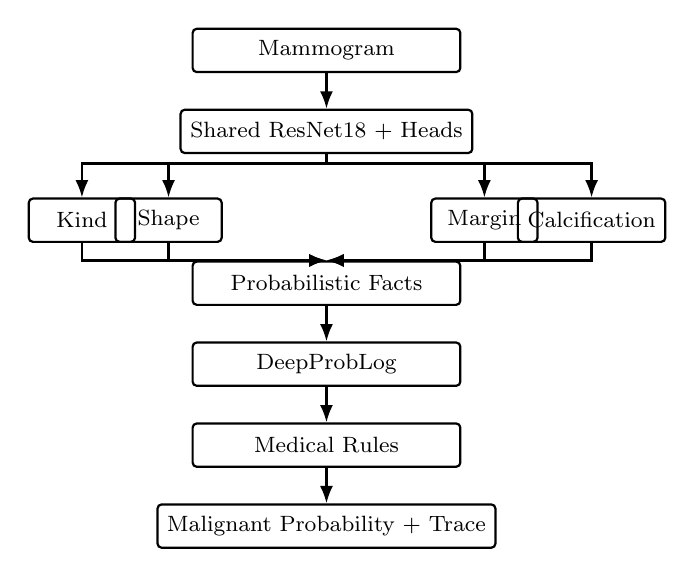
\begin{tikzpicture}[
  font=\footnotesize,
  node distance=0.45cm and 0.22cm,
  box/.style={
    draw,
    rounded corners=1.5pt,
    align=center,
    inner sep=3.5pt,
    minimum height=0.55cm,
    thick
  },
  concept/.style={
    box,
    minimum width=1.35cm
  },
  main/.style={
    box,
    minimum width=3.4cm
  },
  arr/.style={
    -{Latex[length=2.2mm]},
    thick
  }
]
  \node[main] (mammo) {Mammogram};
  \node[main, below=of mammo] (nn) {Shared ResNet18 + Heads};
  \node[concept, below left=0.55cm and 0.55cm of nn] (kind) {Kind};
  \node[concept, below left=0.55cm and -0.55cm of nn] (shape) {Shape};
  \node[concept, below right=0.55cm and -0.55cm of nn] (margin) {Margin};
  \node[concept, below right=0.55cm and 0.55cm of nn] (calc) {Calcification};
  \node[main, below=1.35cm of nn] (facts) {Probabilistic Facts};
  \node[main, below=of facts] (dpl) {DeepProbLog};
  \node[main, below=of dpl] (rules) {Medical Rules};
  \node[main, below=of rules] (out) {Malignant Probability + Trace};

  \draw[arr] (mammo) -- (nn);
  \draw[arr] (nn.south) -- ++(0,-0.12) -| (kind.north);
  \draw[arr] (nn.south) -- ++(0,-0.12) -| (shape.north);
  \draw[arr] (nn.south) -- ++(0,-0.12) -| (margin.north);
  \draw[arr] (nn.south) -- ++(0,-0.12) -| (calc.north);
  \draw[arr] (kind.south) |- (facts.north);
  \draw[arr] (shape.south) |- (facts.north);
  \draw[arr] (margin.south) |- (facts.north);
  \draw[arr] (calc.south) |- (facts.north);
  \draw[arr] (facts) -- (dpl);
  \draw[arr] (dpl) -- (rules);
  \draw[arr] (rules) -- (out);
\end{tikzpicture}
\caption{Overview of the neuro-symbolic breast cancer diagnosis framework. An ImageNet-pretrained ResNet18 trunk feeds four concept heads (lesion kind, shape, margin, calcification); DeepProbLog reasons over those uncertain facts with medical rules to produce a malignant probability and a readable decision trace.}
\label{fig:architecture}
\end{figure}

\subsection{Neural Visual Concept Extraction}
\label{sec:concepts}

The neural model transforms raw image information into clinically meaningful visual concepts, each with an associated probability:
\begin{center}
\small
Image $\rightarrow$ Shared ResNet18 + concept heads $\rightarrow$ $\{\mathrm{lesion\_kind},\;\mathrm{shape},\;\mathrm{margin},\;\mathrm{calcification}\}$.
\end{center}
This differs from a direct mapping $\mathrm{Image}\rightarrow\mathrm{Malignant/ non-Malignant}$ decision. Perception uses a single ImageNet-pretrained ResNet18 trunk~\cite{he2016resnet} with four linear heads (Softmax outputs). Grayscale ROI patches are fed to three channels (RGB) and ImageNet-normalized???. The trunk is frozen for a short head-only warmup, then fine-tuned at a lower learning rate than the heads. The working concept inventory is lesion kind (mass vs.\ calcification), mass shape (regular / irregular / unknown), mass margin (circumscribed / spiculated / other / unknown), and calcification type (absent / typically benign / suspicious), aligned with BI-RADS terminology where annotations permit~\cite{acr2013birads,lee2017cbis}.

The diagnostic target is binary malignancy. In CBIS-DDSM the original pathology field typically has three values: malignant, benign, and benign-without-callback (benign with no additional follow-up indicated). Any label other than malignant is mapped to the negative class. This merges the two non-malignant categories and is a simplifying assumption, not a claim that those categories are clinically identical.

\subsection{Probabilistic Logic Representation}
\label{sec:problog}

Because concept extraction is imperfect, the symbolic component reasons over uncertain evidence rather than treating neural predictions as absolute truths. Neural outputs are neural predicates parameterized by the vision models~\cite{deraedt2007problog,manhaeve2018deepproblog}. DeepProbLog supplies probabilities from those networks, applies logical rules relating concepts to diagnostic hypotheses, and computes the success probability of the query malignant(X). The motivation is joint handling of perception, uncertainty, probabilistic reasoning, and symbolic knowledge---not replacing ordinary conditionals with equivalent Prolog.

\subsection{Medical Knowledge and Rule Representation}
\label{sec:knowledge}

The symbolic knowledge base uses verified domain terminology inspired by BI-RADS~\cite{acr2013birads}. The working program gates evidence by lesion kind so that mass descriptors do not fire on calcifications and suspicious calcification does not fire on masses:

\begin{itemize}
\item malignant if mass and irregular shape;
\item malignant if mass and spiculated margin;
\item malignant if calcification and suspicious calcification type.
\end{itemize}

These rules are a computational working program, not official BI-RADS criteria. Keeping knowledge declarative means a mistaken rule can be rewritten without relabeling images; an early version that treated any calcification as malignant evidence collapsed to always-malignant predictions, and gating by lesion kind restored a usable operating point.

\subsection{Neuro-Symbolic Inference}
\label{sec:inference}

The concept networks learn from images; the symbolic model encodes domain knowledge; and DeepProbLog combines probabilistic neural outputs with logical reasoning~\cite{manhaeve2021neural}. Gradients propagate through ExactEngine inference to update the concept nets. For each case the pipeline reports $P(\mathrm{malignant})$, the concept probabilities, the approximate strength of each rule body, and the strongest rule. That trace is the interpretability mechanism studied in Section~\ref{sec:results}: it shows \emph{how} the decision was formed, not only whether it was correct. Reasoning traces support inspectability; they do not by themselves guarantee clinically adequate explanations.

\section{Experimental Setup}
\label{sec:experiments}

\subsection{Dataset}
\label{sec:dataset}

The working dataset is CBIS-DDSM~\cite{lee2017cbis}. BUSI~\cite{aldhabyani2020busi} remains a candidate for later comparison. Mass and calcification tables are merged. After that merge, some patients appear in both official train and test splits; those patients are assigned entirely to train to prevent data leakage. As stated in Section~\ref{sec:concepts}, pathology is reduced to a binary label by treating benign and benign-without-callback as a single negative class. This is a simplifying assumption. Table~\ref{tab:dataset} reports the resulting split sizes.

\begin{table}[!t]
\caption{CBIS-DDSM split used in this study (patient-disjoint after leakage fix).}
\label{tab:dataset}
\centering
\small
\begin{tabular}{@{}lccc@{}}
\toprule
Split & Rows & Patients & Malignant rate \\
\midrule
Train & 2462 & 1060 & 0.414 \\
Validation & 462 & 188 & 0.392 \\
Test & 644 & 318 & 0.399 \\
\bottomrule
\end{tabular}
\end{table}

\subsection{Neural Model Training}
\label{sec:neural}

Concept perception uses an ImageNet-pretrained ResNet18~\cite{he2016resnet} shared trunk with four heads (lesion kind
; 2 classes, shape: 3 classes, margin 4 classes, calcification type: 3 classes). CBIS cropped ROI images are already lesion-centered patches of the full mammogram; each ROI is turned into one fixed $224\times 224$ tensor by random resized crop on train and center crop on validation/test. Grayscale inputs are repeated to three channels and ImageNet-normalized. Geometric augmentation (horizontal flip, small rotation, and mild affine perturbation) is applied to training images only. Because malignant cases are the minority ($\approx 41\%$ of train), augmentation is class-balanced: both classes are expanded to $4329$ training images ($8658$ total).

Before DeepProbLog training, the trunk and heads receive a supervised concept warm-up: eight epochs of class-weighted cross-entropy on the CSV labels for lesion kind, shape, margin, and calcification type (inverse-frequency weights; trunk frozen for the first two warm-up epochs, then fine-tuned at $0.1\times$ the head learning rate). The warmed networks are then fine-tuned for 15 epochs through DeepProbLog ExactEngine at learning rate $3\times 10^{-4}$ and batch size $2$.

A matched end-to-end ResNet18 malignant/benign binary classifier is trained on the same tensors and splits (no DeepProbLog) as Baseline~1. Decision thresholds for both DeepProbLog and the baseline are chosen on validation (including a high-sensitivity target of $0.80$) and applied unchanged to testing.

\subsection{DeepProbLog Configuration}
\label{sec:dplconfig}

Neural predicates supply lesion\_kind, shape, margin, and calc. Symbolic rules gate mass evidence and calcification evidence by lesion kind, as in Section~\ref{sec:knowledge}. The diagnostic query is malignant(X). These rules are a computational working program and are not presented as official BI-RADS criteria. Training jointly updates the concept heads (and, after warmup, the shared trunk) through the probabilistic program.

\subsection{Implemented Architectures}
\label{sec:Implemented Architectures}
Two architectures have been implemented:
\begin{itemize}
\item \textbf{Baseline:} Pure ResNet18 image classifier (same preprocess and splits; no DeepProbLog).

\item \textbf{Proposed architecture:} Shared ResNet18 concepts + DeepProbLog + symbolic medical knowledge.
\end{itemize}

\subsection{Evaluation Metrics}
\label{sec:metrics}

Reported metrics are accuracy, precision, sensitivity, specificity, F1 for both classes and their macro average, and ROC-AUC. The decision threshold on $P(\mathrm{malignant})$ is chosen on validation only. The primary operating point targets validation sensitivity $\geq 0.80$, reflecting the clinical priority of catching malignancies even when that lowers specificity; a more balanced macro-F1 cut-off and the conventional $0.5$ baseline cut-off are also reported. Interpretability---the reason DeepProbLog is used---is assessed qualitatively via reasoning traces on selected true/false positive and negative cases: each trace lists concept probabilities, rule-body strengths, the strongest rule, and the final decision.

\section{Results and Discussion}
\label{sec:results}

Results are reported on the patient-disjoint CBIS-DDSM test split ($n=644$). Table~\ref{tab:comparison} compares DeepProbLog with the pure ResNet18 baseline. Ranking quality is essentially matched: DeepProbLog test ROC-AUC is $0.752$ versus $0.746$ for the baseline. The important difference appears at the operating point.

We deliberately choose the decision threshold on validation to target high sensitivity ($\geq 0.80$), because missing a malignant case is clinically more costly than an extra false alarm. Under that protocol DeepProbLog reaches test sensitivity $0.798$ with specificity $0.558$ (threshold $0.55$). A more balanced validation macro-F1 cut-off ($0.60$) yields sensitivity $0.716$ and specificity $0.633$. The baseline at the conventional $0.5$ cut-off has higher specificity ($0.755$) but only sensitivity $0.591$; even when pushed toward higher recall (fallback threshold $0.44$), it reaches only about $0.61$ sensitivity and never meets the $0.80$ target.

\begin{table}[!t]
\caption{Test-set comparison ($n=644$). Starred thresholds were chosen on validation for sensitivity $\geq 0.80$; dagger marks the validation macro-F1 cut-off. The baseline never reached sensitivity $0.80$ on validation, so its high-sensitivity row uses the fallback Youden threshold. AUC is threshold-free.}
\label{tab:comparison}
\centering
\small
\begin{tabular}{@{}llccccc@{}}
\toprule
Model & Setup & Thr. & Acc. & Sens. & Spec. & AUC \\
\midrule
DPL & ResNet18 + warm-up & $0.55^*$ & $0.654$ & $0.798$ & $0.558$ & $0.752$ \\
DPL & ResNet18 + warm-up & $0.60^\dagger$ & $0.666$ & $0.716$ & $0.633$ & $0.752$ \\
CNN & ResNet18 baseline & $0.50$ & $0.689$ & $0.591$ & $0.755$ & $0.746$ \\
CNN & ResNet18 baseline & $0.44$ & $0.693$ & $0.611$ & $0.747$ & $0.746$ \\
\bottomrule
\end{tabular}
\end{table}

\paragraph{Why sensitivity is higher and specificity is lower.}
This pattern is expected under a high-recall policy, not a failure of DeepProbLog. Lowering the malignancy threshold catches more true malignancies (higher sensitivity) and inevitably labels more benign cases as malignant (lower specificity). DeepProbLog can operate near sensitivity $0.80$ while remaining inspectable; the pure CNN, with similar AUC, does not reach that recall target on the same validation protocol. At a default $0.5$ cut-off the baseline still looks stronger on accuracy and specificity, which is why both operating points are reported: the clinical priority (find malignancies) and the conventional cut-off tell different stories.

Concept agreement on validation (probability of the gold label $\geq 0.5$) is kind $0.905$, shape $0.723$, margin $0.701$, and calcification $0.820$. Margin remains the weakest concept, consistent with remaining false negatives and false positives.

\subsection{How DeepProbLog Exposes the Decision}
\label{sec:traces}

A conventional CNN returns only $P(\mathrm{malignant})$. DeepProbLog returns that probability as the success probability of the query malignant(X), computed from the concept networks through the three rules. For each case the pipeline reports concept probabilities, the approximate strength of each rule body, the strongest rule, and the binary decision. That decomposition is the reason DeepProbLog is used here: explainability through an explicit concept--rule path.

\paragraph{Correct malignant case.}
For validation case P\_00045 (malignant mass), the model gave $P(\mathrm{kind}=\mathrm{mass})=1.000$ and $P(\mathrm{shape}=\mathrm{irregular})=0.983$, so the mass--irregular rule dominated and $P(\mathrm{malignant})=0.983$.

\paragraph{False positive from wrong lesion kind.}
Validation case P\_00061 (benign mass) is instructive: the nets assigned $P(\mathrm{kind}=\mathrm{calcification})=0.990$ and $P(\mathrm{calc}=\mathrm{suspicious})=0.919$, so the calcification rule fired ($P(\mathrm{malignant})=0.910$) despite gold descriptors indicating a mass. The symbolic layer applied the correct rule to incorrect concepts---an error a black-box score would not localize.

\paragraph{Remaining errors are still perception.}
Test false negative P\_00017 is malignant with gold shape regular and margin other, so no malignancy rule should fire strongly from gold labels; the model partially called irregular shape ($0.363$) but stayed below the $0.55$ threshold. Test false positive P\_00032 is a benign mass where irregular shape was over-called ($0.719$) and the mass--irregular rule fired. In both cases the decision path is readable as concept error rather than an opaque logit.
From the above, it can be seen that DeepProbLog provides explainability: predictions decompose into BI-RADS-style concept probabilities and rule firings, so errors can be attributed to named descriptors rather than a single score. Second, performance is competitive with a pure ResNet18 baseline (AUC $0.752$ vs.\ $0.746$), while DeepProbLog uniquely supports a high-sensitivity operating point near $0.80$ recall. Third, the lower specificity at that point is the deliberate cost of prioritizing sensitivity; a more balanced threshold recovers specificity at the expense of some recall. Declarative rules remain editable without relabeling images.

\section{Conclusion}
\label{sec:conclusion}

This paper presented a neuro-symbolic breast cancer diagnosis pipeline whose purpose is explainable decisions, not opaque end-to-end scoring. An ImageNet-pretrained ResNet18 trunk with four concept heads extracts lesion kind, shape, margin, and calcification type; the heads are warmed up with class-weighted cross-entropy on CSV descriptors and then fine-tuned through DeepProbLog ExactEngine with lesion-kind-gated rules inspired by BI-RADS. A matched end-to-end ResNet18 classifier on the same patient-disjoint CBIS-DDSM splits is the accuracy reference.

On the test set, DeepProbLog reaches ROC-AUC $0.752$, essentially matching the baseline ($0.746$). At a validation-chosen high-sensitivity threshold ($0.55$), sensitivity is $0.798$ and specificity $0.558$; a more balanced macro-F1 cut-off ($0.60$) yields sensitivity $0.716$ and specificity $0.633$. The baseline does not attain sensitivity $0.80$ under the same protocol. The higher sensitivity and lower specificity at the primary operating point follow from deliberately prioritizing recall: fewer missed malignancies, at the cost of more false positives---a tradeoff that DeepProbLog makes while still exposing which concepts and rules drove each call.

Unlike an end-to-end CNN that returns only $P(\mathrm{malignant})$, the proposed system reports concept probabilities, rule-body strengths, and the strongest rule. Remaining errors are attributable to under- or over-called BI-RADS descriptors---especially lesion kind, shape, and margin---rather than to opaque logits. Declarative rules remain editable without relabeling images.

Future work includes stronger margin-focused supervision, expert review of reasoning traces, and evaluation on additional datasets such as BUSI.


\bibliographystyle{IEEEtran}
\bibliography{references}

\end{document}
